\documentclass{beamer}
\usefonttheme[onlymath]{serif}
% does not look nice, try deleting the line with the fontenc.
\usepackage[english]{babel}
\usepackage{amsmath}
\usepackage[latin1]{inputenc}
\usepackage{units}
\usepackage{colortbl}
\usepackage{multimedia}
\usepackage{bm}

\mode<presentation>
{
  \usetheme{Boadilla}
  \useoutertheme{infolines}
  \setbeamercovered{transparent} 
}

\newcommand{\Name}{\emph{dynoNet}}

\title[LRU reduction]{Model order reduction of deep structured state-space models: A system-theoretic approach}

%\subtitle{Industrial-scale experimental results\\} % (optional)

\author[]{Marco Forgione, Manas Mejari, and Dario Piga}

\institute[IDSIA]{
	\inst{1}IDSIA Dalle Molle Institute for Artificial Intelligence SUPSI-USI, Lugano, Switzerland 
	} 


\date[]{\today}


\subject{System identification with neural networks}


%% MATH DEFINITIONS %%
\newcommand{\q}{q} % shift operator
\newcommand{\A}{A} % autoregressive polynomial
\newcommand{\ac}{a} % autoregressive polynomial coefficient
\newcommand{\B}{B} % exogenous polynomial
\newcommand{\bb}{b} % exogenous polynomial coefficient
\newcommand{\Gmat}{\mathbb{G}} % transfer function operator in matrix form
\newcommand{\tvec}[1]{\mathbf{#1}}
\newcommand{\mat}[1]{\bm{#1}}
\newcommand{\sens}[1]{\tilde{#1}}
\newcommand{\adjoint}[1]{\overline{#1}}
\newcommand{\loss}{\mathcal{L}}
\newcommand{\pdiff}[2]{\frac{\partial #1}{\partial #2}}
\newcommand{\nsamp}{T}

\newcommand{\conv}{*}
\newcommand{\ccorr}{\star}
%\newcommand{\R}{\mathcal{R}}
%\newcommand{\du}{\delta u}
%\newcommand{\dy}{\delta y}
%\newcommand{\DU}{\Delta U}
%\newcommand{\DY}{\Delta Y}
%\newcommand{\abs}[1]{\left | #1 \right |}
\newcommand{\norm}[1]{\left \lVert #1 \right \rVert}
%\newcommand{\relphantom}[1]{\mathrel{\phantom{#1}}}
%\newenvironment{matrixc}{\begin{array}{c}\left[}{\end{array}\right]}
\DeclareMathOperator*\argmin{arg \, min}
%\DeclareMathOperator*\argmax{arg \, max}
%\DeclareMathOperator*\fit{fit}
%\DeclareMathOperator*\RMSE{RMSE}
%\DeclareMathOperator*\diag{diag}
%\DeclareMathOperator*\diet{diet}
%\DeclareMathOperator*\Risk{Risk}
%\DeclareMathOperator*\Num{Num}
%\DeclareMathOperator*\Den{Den}
%\DeclareMathOperator*\Rat{Rat}
\DeclareMathOperator*\cov{cov}
%\DeclareMathOperator*\Var{Var}
%\DeclareMathOperator*\SSR{SSR}
%\setcounter{MaxMatrixCols}{20}
%\newcommand{\pdiff}[2]{\frac{\partial #1}{\partial #2}}
%\definecolor{mypink1}{rgb}{0.858, 0.188, 0.478}
%\definecolor{olive}{RGB}{85, 107, 47}
\definecolor{orange}{RGB}{204, 85, 0}

%\definecolor{mypink3}{cmyk}{0, 0.7808, 0.4429, 0.1412}
%\definecolor{mygray}{gray}{0.6}
%\definecolor{olivegreen}[RGB]{85, 107, 47}

\newcommand{\K}{K}
\newcommand{\M}{M}
\newcommand{\Mo}{M_o}
\newcommand{\So}{S_o}
\newcommand{\Smod}{S}
\newcommand{\parcolor}[1]{{\color{orange}#1}}
\newcommand{\Ts}{T_s^{\rm MPC}}
\newcommand{\cites}[1]{\begin{small}(#1)\end{small}}
%\newcommand{\Ts}{T_s}

\definecolor{darkgreen}{RGB}{20,150,50}
\definecolor{acq}{RGB}{119, 172, 48}
\definecolor{true}{RGB}{162, 20, 47}
\definecolor{surr}{RGB}{0, 114, 189}

\usepackage{listings}
% Default fixed font does not support bold face
\DeclareFixedFont{\ttb}{T1}{txtt}{bx}{n}{12} % for bold
\DeclareFixedFont{\ttm}{T1}{txtt}{m}{n}{12}  % for normal

\newcommand\pythonstyle{\lstset{
language=Python,
basicstyle=\ttb\tiny,
otherkeywords={self},             % Add keywords here
keywordstyle=\tiny\color{deepblue},
emph={MyClass,__init__},          % Custom highlighting
emphstyle=\ttb\color{deepred},    % Custom highlighting style
stringstyle=\color{deepgreen},
frame=tb,                         % Any extra options here
showstringspaces=false,            %
numberstyle=\footnotesize,
}}

\lstnewenvironment{python}[1][]
{
\pythonstyle
\lstset{#1}
}
{}

\newcommand{\book}{
\includegraphics[width=10pt]{img/proceeding-logo.jpg}}
\newcommand{\github}{
\includegraphics[width=10pt]{img/github-logo.jpg}}

\usepackage{multirow}
\usepackage{adjustbox}
\usepackage{booktabs}
\usepackage{caption}

\begin{document}

\begin{frame}
  \titlepage
\end{frame}

\begin{frame}{Deep structured state-space models}
Growing interest within the machine-learning community. They dominate \structure{long-range} sequence learning where Transformers suffer the $\mathcal{O}(N^2)$ scaling.
\vskip 1em 

\begin{itemize}
%\item They dominate \structure{very long-range} sequence learning tasks where Transformers suffer the $\mathcal{O}(T^2)$ scaling
\item Interconnection of \structure{linear dynamical} systems with \structure{static non-linearities} (and Normalization layers, skip connection, ...)
\item The architecture should \structure{ring a bell} to sysid researchers.
\end{itemize}

\only<1>{
\vskip 7em
}
\only<2->{
\vskip 1em
The classic \structure{block-oriented} modeling framework.
\begin{columns}
\column{.2\textwidth}
 \begin{figure}
 \footnotesize  Wiener
 \vskip .5em
 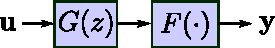
\includegraphics[width=\textwidth]{img/wiener.pdf}
 \end{figure}
\column{.2\textwidth}
 \begin{figure}
 \footnotesize Hammerstein
 \vskip .5em
 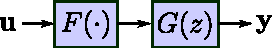
\includegraphics[width=\textwidth]{img/hammer.pdf}
 \end{figure}
 \column{.3\textwidth}
 \begin{figure}
 \footnotesize Wiener-Hammerstein
 \vskip .5em
 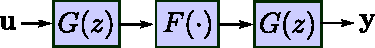
\includegraphics[width=\textwidth]{img/wiener_hammerstein.pdf}
 \end{figure}
\end{columns}
%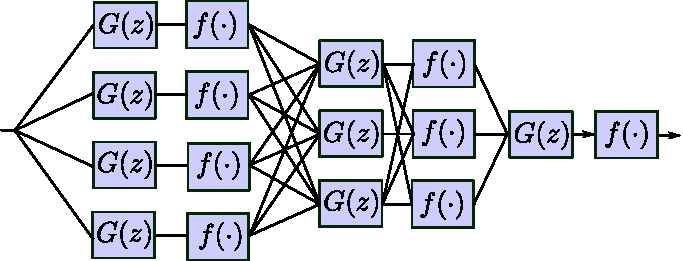
\includegraphics[scale=.2]{img/generic_layer.pdf}
\begin{itemize}
 	\item[\book]
 		\begin{tiny}
 	\structure{E.W. Bai, F. Giri}
 									Block-oriented nonlinear system identification. \emph{Springer}, 2010
 		\end{tiny}					
\end{itemize}
}
\end{frame}

\begin{frame}[fragile]{The dynoNet architecture}
LTI blocks for deep learning also in our 2021 \structure{dynoNet} architecture
\vskip 1em
\begin{columns}
 \column{.5\textwidth}
 \centering
 \Name \ architecture
\begin{figure}
 \vskip 0em
 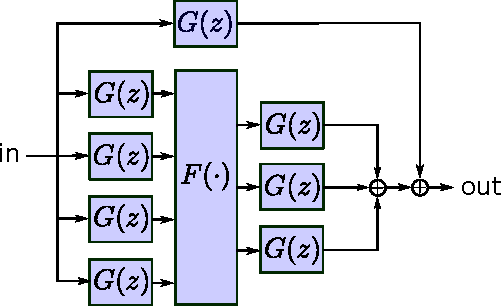
\includegraphics[width=.8\textwidth]{img/generic_dynonet.pdf}
\end{figure}
 \column{.5\textwidth}
 \centering
 \vskip -.5em
 Python code
  \begin{tiny}
\begin{lstlisting}[language=python]


G1 = LinearMimo(1,  4, ...) # a SIMO tf
F = StaticNonLin(4, 3, ...) # a static NN
G2 = LinearMimo(3, 1, ...) # a MISO tf
G3 = LinearSiso(1, 1, ...) # a SISO tf
 
def model(in_data):  
    y1 = G1(in_data)
    z1 = F(y1) 
    y2 = G2(z1)
    out = y2 + G3(in_data)
    
\end{lstlisting}
\end{tiny}
\end{columns}
\vskip 1.5em
%It enables training of arbitrary linear/non-linear combinations.
% \vskip 1em 

\begin{itemize}
 	\item[\book]
 		\begin{tiny}
 	\structure{M. Forgione and D.Piga.}
 									\emph{dynoNet}: A Neural Network architecture for learning dynamical systems.
 									\vskip -1em
 									\emph{International Journal of Adaptive Control and Signal Processing}, 2021
 		\end{tiny}
\end{itemize}
\only<1>{\vskip 4em}
\only<2->{
\structure{Differentiable transfer functions} are now also in the \href{https://pytorch.org/audio/main/generated/torchaudio.functional.lfilter.html}{\texttt{torchaudio}} library. 
%\\
%dynoNet included in the documentation of {\texttt{torchaudio.lfilter}}.
\begin{itemize}
 	\item[\book]{\begin{tiny}https://pytorch.org/audio/main/generated/torchaudio.functional.lfilter.html\end{tiny}}					
\end{itemize}
}
\end{frame}

\begin{frame}{Deep Structured State-Space Model Architecture}
%Very close to dynoNet. Main differences:
\begin{itemize}
\item Architecture with normalization layers, skip connections, (dropout). 
\item State-space parameterization of the linear dynamical system
\end{itemize}
\begin{figure}
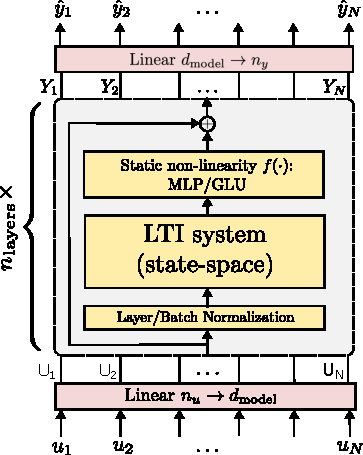
\includegraphics[scale=.5]{img/s4_architecture.pdf}
\end{figure}
Focus on making the LTI system   learning \structure{fast and well-posed}.
\begin{itemize}
 	\item[\book]
 		\begin{tiny}
 	\structure{A. Gu, K. Goel, C. R\'e.}
 									Efficiently Modeling Long Sequences with Structured State Spaces. \emph{ICLR}, 2022		
 		\end{tiny}		
\end{itemize}
\pause
\vskip 1em
Our idea: bring in \structure{model order reduction} to simplify these architectures!
\end{frame}


\begin{frame}{Deep Linear Recurrent Unit}
We consider the deep LRU architecture recently introduced by DeepMind:
\begin{itemize}
 	\item[\book]
 		\begin{tiny}
 	\structure{A. Orvieto et al.}
 									Resurrecting Recurrent Neural Networks for Long Sequences. \emph{ICML}, 2023 				
 		\end{tiny}		
\end{itemize}
%\vskip 1em
\begin{columns}[t]
\column{.25\textwidth}
\begin{figure}
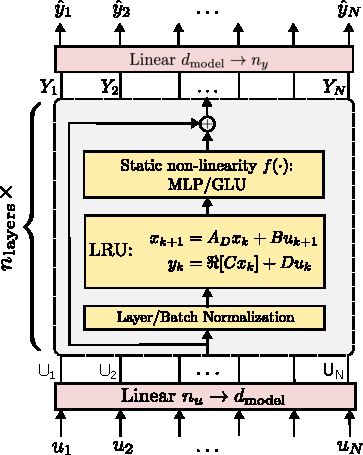
\includegraphics[scale=.5]{img/lru_architecture.pdf}
\end{figure}
\column{.75\textwidth}
\begin{itemize}
\item Discrete-time, MIMO LTI system
\item Complex diagonal state-transition matrix $A_D$:
\vskip -0.5em
$$A_D = \textrm{diag}(\lambda_1, \lambda_2, \dots, \lambda_{n_x})$$
\vskip -1.5em
\item Stable parameterization with $|\lambda_i| < 1$
\item Implementation with either:
\begin{itemize}
\item $\mathcal{O}(N)$ sequential ops (standard recursion) 
\item $N$ \structure{parallel} jobs, $\mathcal{O}(\log N)$ ops each \structure{(parallel scan)}
\end{itemize}
\end{itemize}
\end{columns}
\vskip 1em

\pause
Our idea: further exploit the \structure{diagonal structure} for model order reduction.
\end{frame}

\begin{frame}{Model Order Reduction}
Consider a LTI state-space system partitioned as:
\begin{align*}\label{eq:ss_partitioned_a}
    \begin{bmatrix}
    x_{1}(k)\\
    x_{2}(k)
    \end{bmatrix}
    &=
    \begin{bmatrix}A_{11} & A_{12} \\ A_{21} & A_{22} \end{bmatrix}     
    \begin{bmatrix}
    x_{1}(k-1)\\
    x_{2}(k-1)
    \end{bmatrix} + \begin{bmatrix}B_1\\B_2 \end{bmatrix} u(k), \\
    y(k) &= \begin{bmatrix}C_1\;\; C_2\end{bmatrix} \begin{bmatrix}x_{1}(k)\\ x_{2}(k) \end{bmatrix} + D u(k),
\end{align*}
The states $x_2$ can be removed by:
\begin{itemize}
\item \textbf{T}runcation $\Rightarrow$ keep $(A_{11}, B_{1}, C_{1}, D)$
\item \textbf{S}ingular \textbf{P}erturbation $\Rightarrow$ solve for $x_{2}(k) = x_{2}(k-1)$
%\begin{small}
%\begin{align*}
%    A_r &= A_{11} + A_{12}(I - A_{22})^{-1}A_{21}\\
%    B_r &= B_1 + A_{12} (I - A_{22})^{-1} B_2 \\
%    C_r &= C_1 + C_2 (I - A_{22})^{-1} A_{21} \\
%    D_r &= C_2 (I - A_{22})^{-1} B_2 + D.
%\end{align*}
%\end{small}
%\begin{footnotesize}
%$$
%    (A_{11} + A_{12}(I - A_{22})^{-1}A_{21}, B_1 + A_{12} (I - A_{22})^{-1} B_2, C_1 + C_2 (I - A_{22})^{-1} A_{21}, C_2 (I - A_{22})^{-1} B_2 + D).
%$$
%\end{footnotesize}
\end{itemize}
\pause
Reduction is often applied to systems in 
\begin{itemize}
\item \textbf{M}odal form ($A$ diagonal, states sorted from slowest to fastest)
\item \textbf{B}alanced form (states sorted for decreasing Hankel singular values)
\end{itemize}
%\pause
\vskip 1em
\pause
We tested all combinations: MT, MSP, BT, BSP.
\end{frame}

\begin{frame}{Regularization for MOR}
Regularization introduced to enhance the MOR:
\begin{align*}
\theta^* =  \arg\min_{\theta \in \Theta}  & \frac{1}{N}\sum_{k=1}^N \left(y_k - \hat{y}_k(\theta) \right)^2 +  \gamma \mathcal{R}(\theta),  
\end{align*}
\vskip -1.0em
\begin{columns}
\column{.48\textwidth}
\begin{block}{Modal $\ell_1$}
\begin{equation*}
    \mathcal{R}(\theta) = \sum_{j=1}^{n_x} |\lambda_j|
\end{equation*}
\begin{itemize}
\item Push some modes $\lambda_j$ towards 0
%\item Rationale: fast modes can often be neglected
\item Tailored for modal reduction MT/MSP
%\item Directly applicable
\end{itemize}
\end{block}
\column{.48\textwidth}
\begin{block}{Hankel nuclear norm (HNN)} 
\begin{equation*}
	\mathcal{R}(\theta) = \sum_{j=1}^{n_x} \sigma_j
\end{equation*}
\begin{itemize}
\item Push some HSV $\sigma_j$  towards 0
\item Tailored for balanced reduction BT/BSP
%\item Directly applicable
\end{itemize}
\end{block}
\end{columns}
\vskip .5em
\pause
\begin{itemize}
\item Modal $\ell_1$ efficient ($\lambda_j$ are on the diagonal of $A_D$)
\item HNN also efficient exploiting diagonal $A_D$ structure\dots
\end{itemize}
\end{frame}

\begin{frame}{Hankel nuclear norm minimization}
%Let us denote as $G$ and $G_r$ the original and reduced system.\\
\begin{itemize}
\item The HNN $\sum_{j=1}^{n_x} \sigma_j$ is a convex approximation to the McMillan degree of a linear system $G$ (minimium realization order). 
\item The choice of HNN regularization is further motivated by the bound:
\begin{equation*}
\norm{G-G_r}_{\mathcal{H}_\infty} \leq 2\sum \limits_{j=r+1}^{n_x}\sigma_j,
\end{equation*}
valid when $G_r$ is obtained with balanced reduction methods BT/BSP
\end{itemize}
\pause
\vskip 2em
If we push some HSVs of $G$ towards zero, we can then then find an (almost) equivalent reduced  $G_r$ with balanced reduction methods!
\end{frame}


\begin{frame}{Example}

Experiments on the F16 ground vibration \href{https://research.tue.nl/en/datasets/f-16-aircraft-benchmark-based-on-ground-vibration-test-data}{benchmark}. 
\vskip 1em
\begin{columns}
\column{.45\textwidth}
Deep LRU with:
\begin{itemize}
 \item $n_{\rm layers}=6$  layers
 \item $n_x=100$ states per layer
 \item $d_{\rm model}=50$ units per layer
 \item Layer Normalization
 \item MLP non-linearity

\end{itemize}
\column{.55\textwidth}
\begin{center}
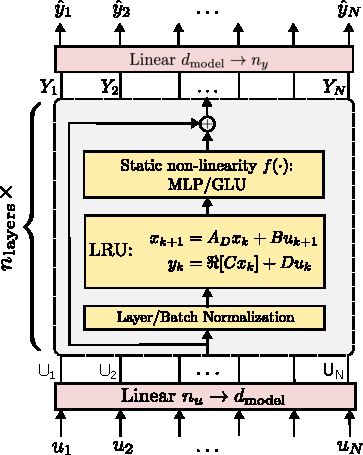
\includegraphics[scale=.7]{img/lru_architecture.pdf}
\end{center}
\end{columns}
%\vskip .2em
%Results on test set \texttt{FullMSine\_Level6\_Validation}
%\begin{table}[ht]
%\centering
%%\captionsetup{justification=centering} % Centering captions
%\small % Reduced font size
%\setlength{\tabcolsep}{4pt} % Reduced column padding
%\adjustbox{scale=0.7}{
%\begin{tabular}{@{}l*{9}{c}@{}} % Adjusting column alignment
%\toprule
%\multirow{2}{*}{Regularization} & \multicolumn{3}{c}{Channel 1} & \multicolumn{3}{c}{Channel 2} & \multicolumn{3}{c}{Channel 3} \\
%\cmidrule(lr){2-4} \cmidrule(lr){5-7} \cmidrule(lr){8-10}
%& {\emph{fit}} & {RMSE} & {NRMSE} & {\emph{fit}} & {RMSE} & {NRMSE} & {\emph{fit}} & {RMSE} & {NRMSE} \\
%\midrule
%No reg. & 86.5 & 0.180 & 0.134 & 90.0 & 0.167 & 0.099  & 76.2 & 0.368 & 0.237 \\
%Modal $\ell_1$ & 85.4 & 0.195 & 0.145 & 89.8 & 0.171 & 0.102 & 74.5 & 0.395 & 0.254 \\
%Hankel norm & 85.8 & 0.190 & 0.142 & 89.0 & 0.185 & 0.110 & 75.5 & 0.379 & 0.245 \\
%\bottomrule
%\end{tabular}
%}
%\caption{Performance of the SSM trained with different regularization methods.}
%\end{table}
%\vskip .2em
%\pause
%In line with literature. Regularization has a large effect on the LTI blocks!
\vskip 2em
\begin{itemize}
\item[\github] \url{https://github.com/forgi86/lru-reduction}
\end{itemize}
\end{frame}

\begin{frame}{Nominal results}
\begin{columns}
\column{.5\textwidth}
Training repeated with:
\begin{itemize}
 \item No regularization
 \item Modal $\ell_1$ regularization
 \item Hankel norm regularization.
\end{itemize}

\column{.5\textwidth}
\begin{center}
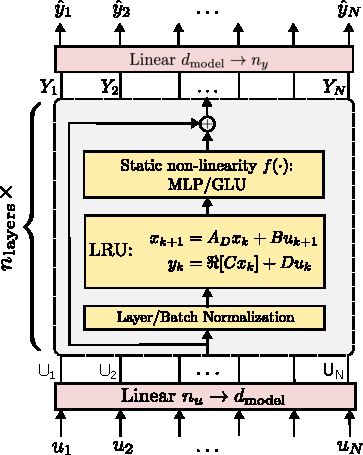
\includegraphics[scale=.5]{img/lru_architecture.pdf}
\end{center}
\end{columns}

\pause
\vskip 1em
Results on test set \texttt{FullMSine\_Level6\_Validation}:
\begin{table}[ht]
\centering
%\captionsetup{justification=centering} % Centering captions
\small % Reduced font size
\setlength{\tabcolsep}{4pt} % Reduced column padding
\adjustbox{scale=0.7}{
\begin{tabular}{@{}l*{9}{c}@{}} % Adjusting column alignment
\toprule
\multirow{2}{*}{Regularization} & \multicolumn{3}{c}{Channel 1} & \multicolumn{3}{c}{Channel 2} & \multicolumn{3}{c}{Channel 3} \\
\cmidrule(lr){2-4} \cmidrule(lr){5-7} \cmidrule(lr){8-10}
& {\emph{fit}} & {RMSE} & {NRMSE} & {\emph{fit}} & {RMSE} & {NRMSE} & {\emph{fit}} & {RMSE} & {NRMSE} \\
\midrule
No reg. & 86.5 & 0.180 & 0.134 & 90.0 & 0.167 & 0.099  & 76.2 & 0.368 & 0.237 \\
Modal $\ell_1$ & 85.4 & 0.195 & 0.145 & 89.8 & 0.171 & 0.102 & 74.5 & 0.395 & 0.254 \\
Hankel norm & 85.8 & 0.190 & 0.142 & 89.0 & 0.185 & 0.110 & 75.5 & 0.379 & 0.245 \\
\bottomrule
\end{tabular}
}
%\caption{Performance of the SSM trained with different regularization methods.}
\end{table}

%\vskip .2em
%\pause
In line with literature. Regularization has a large effect on the LTI blocks!

\end{frame}

\begin{frame}
\begin{figure}[ht]
    \centering
    No regularization: eigenvalues magnitude (top) and HSV (bottom)\\
    %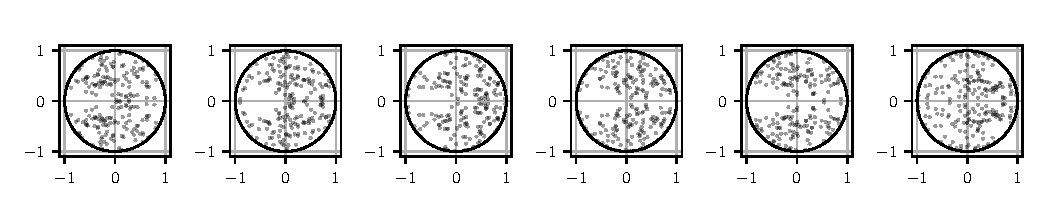
\includegraphics[scale=.99]{figures/F16/ckpt_large_no_reg_eigs_complex.pdf}
    %\vskip -1em
    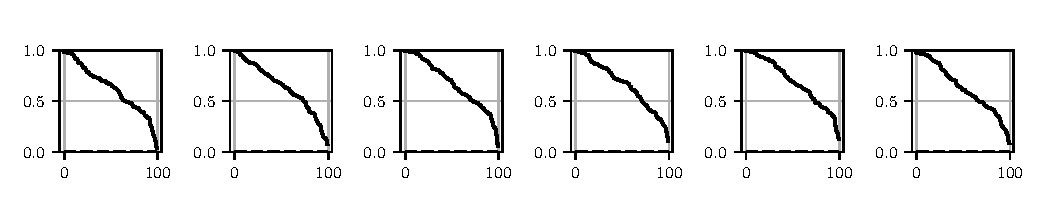
\includegraphics[scale=.5]{img/ckpt_large_no_reg_eigs_abs.pdf}
    \vskip -.5em
    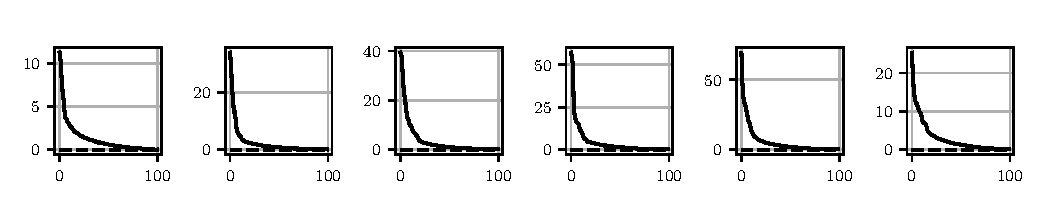
\includegraphics[scale=.5]{img/ckpt_large_no_reg_hankel.pdf}
    % \caption{No regularization: complex eigenvalues in the unit circle (top), eigenvalues magnitude (middle) and Hankel singular values (bottom).}
\end{figure}
\begin{figure}[ht]
    \centering
    Modal $\ell_1$ regularization: eigenvalues magnitude (top) and HSV (bottom)\\
    %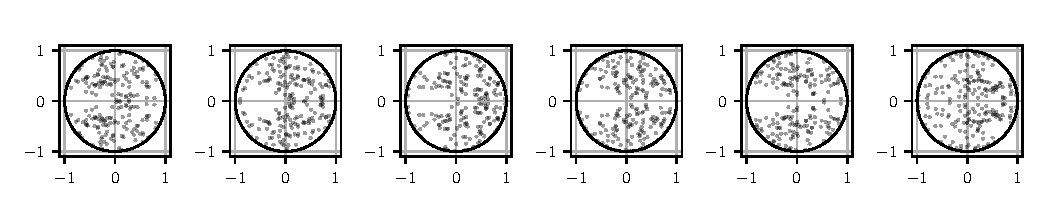
\includegraphics[scale=.99]{figures/F16/ckpt_large_no_reg_eigs_complex.pdf}
    %\vskip -1em
    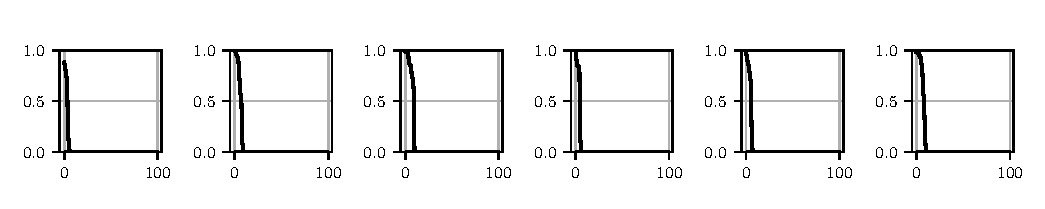
\includegraphics[scale=.5]{img/ckpt_large_reg_modal_eigs_abs.pdf}
    \vskip -.5em
    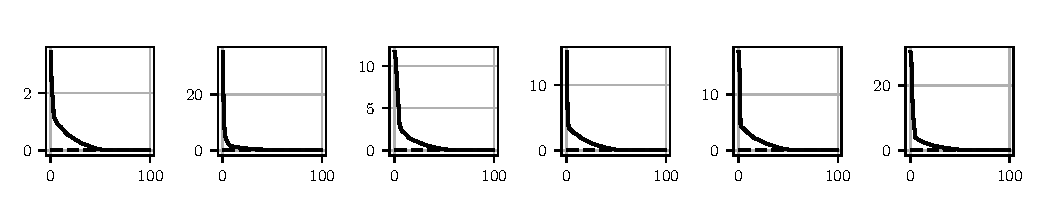
\includegraphics[scale=.5]{img/ckpt_large_reg_modal_hankel.pdf}
    % \caption{No regularization: complex eigenvalues in the unit circle (top), eigenvalues magnitude (middle) and Hankel singular values (bottom).}
\end{figure}
\end{frame}

\begin{frame}
\begin{figure}[ht]
    \centering
    No regularization: eigenvalues magnitude (top) and HSV (bottom)\\
    %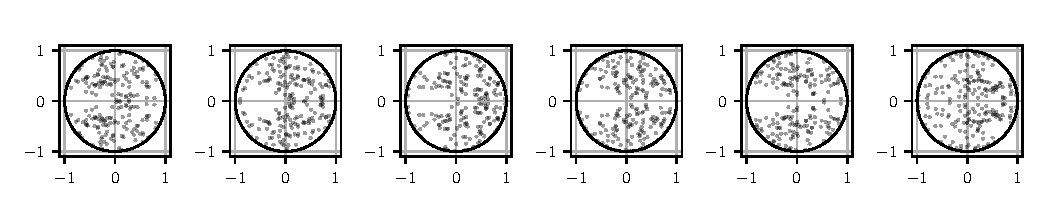
\includegraphics[scale=.99]{figures/F16/ckpt_large_no_reg_eigs_complex.pdf}
    %\vskip -1em
    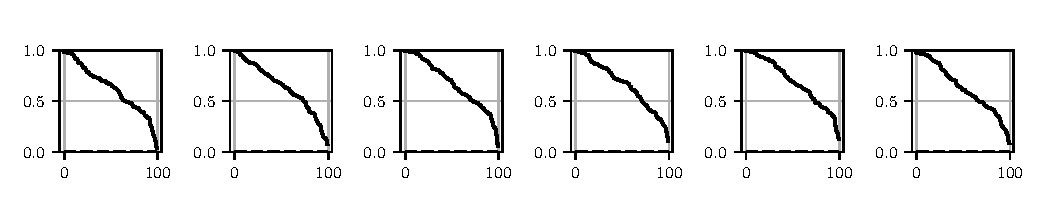
\includegraphics[scale=.5]{img/ckpt_large_no_reg_eigs_abs.pdf}
    \vskip -.5em
    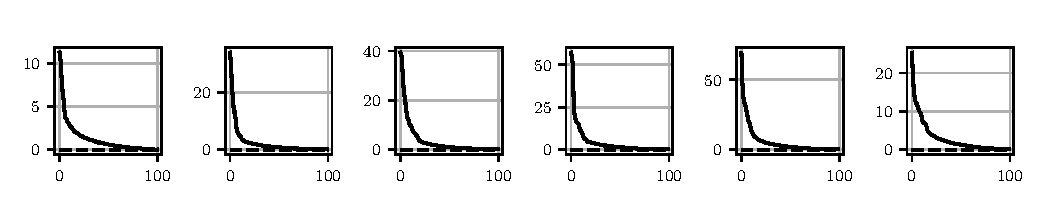
\includegraphics[scale=.5]{img/ckpt_large_no_reg_hankel.pdf}
    % \caption{No regularization: complex eigenvalues in the unit circle (top), eigenvalues magnitude (middle) and Hankel singular values (bottom).}
\end{figure}
\begin{figure}[ht]
    \centering
    HNN regularization: eigenvalues magnitude (top) and HSV (bottom)\\
    %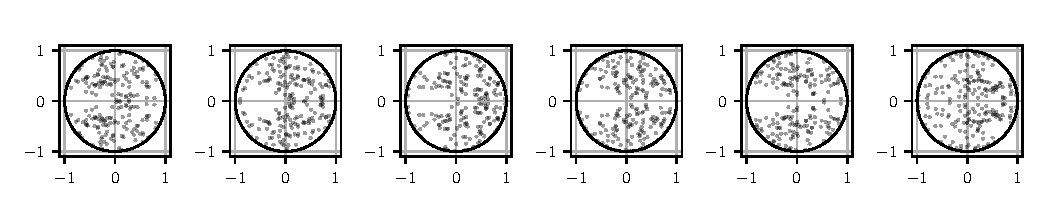
\includegraphics[scale=.99]{figures/F16/ckpt_large_no_reg_eigs_complex.pdf}
    %\vskip -1em
    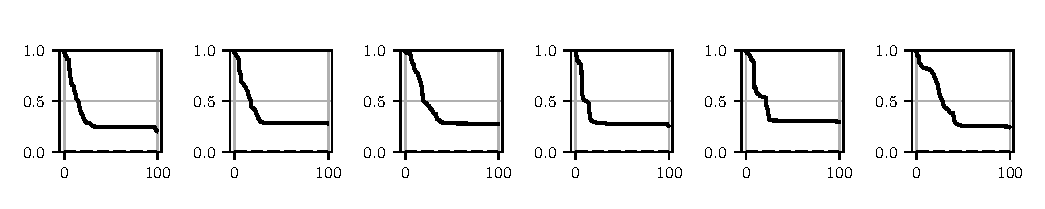
\includegraphics[scale=.5]{img/ckpt_large_reg_hankel_eigs_abs.pdf}
    \vskip -.5em
    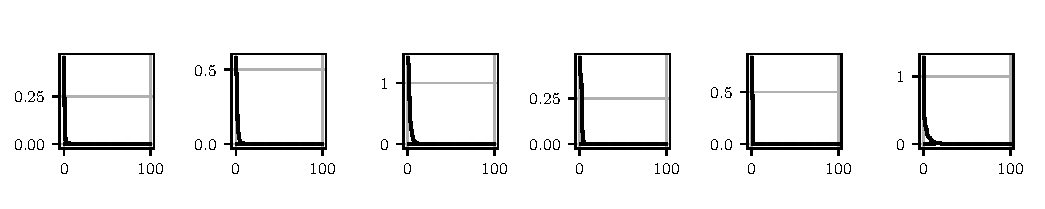
\includegraphics[scale=.5]{img/ckpt_large_reg_hankel_hankel.pdf}
    % \caption{No regularization: complex eigenvalues in the unit circle (top), eigenvalues magnitude (middle) and Hankel singular values (bottom).}
\end{figure}
\end{frame}


\begin{frame}{Model Order Reduction}
Performance of all Regularization/Reduction combinations assessed.
\vskip 2em
\begin{columns}
\column{.5\textwidth}
\begin{table}%[htbp]
	\small
	\adjustbox{scale=0.7}{
    \centering
    \begin{tabular}{@{}lllll@{}}
    \toprule
    & \multicolumn{4}{c}{Reduction Method} \\ \cmidrule(lr){2-5}
    Regularization Method & BT & BSP & MT & MSP \\ \midrule
    No Regularization & 28 & 43 & 3 & 35 \\
    Modal $\ell_1$& 56 & 73 & 0 & \textbf{91} \\
    Hankel nuclear norm& 89 & \textbf{91} & 18 & 76 \\ \bottomrule
    \end{tabular}
}
\caption{\small Number of states eliminated s.t. performance decrease is less than 1\%}
\end{table}
\column{.5\textwidth}
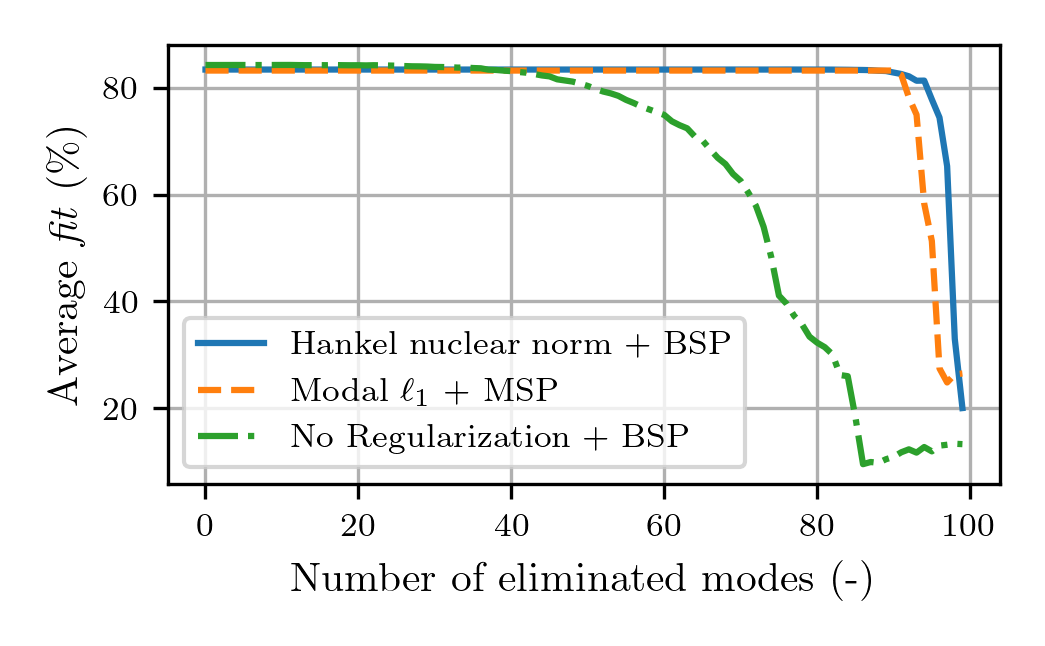
\includegraphics[width=\columnwidth]{img/MOR_regularization.png}
\end{columns}
\vskip 1em
\begin{itemize}
\item Best results with Hankel nuclear norm + balanced singular perturbation and modal $\ell_1$ + modal singular perturbation 
\item Without regularization, MOR is significantly less effective
\end{itemize}
\end{frame}

\begin{frame}{Conclusions \& future research}
Preliminary efforts to improve deep SSMs with System Theoretic tools.\\
MOR + tailor-made regularization to reduce state dimensionality.
\vskip 1em
\pause
Future research:
\begin{itemize}
\item More extensive simulations (e.g., effect of the regularization strength)
\item Other model order reduction (e.g., Kyrilov-based) and regularizers
\item Reduction also of layers and channels
\item Application to other models where LTI blocks are key, e.g.
\begin{itemize}
\item Koopman-based
\item dynoNet
\item Other deep SSMs
\end{itemize}
%\item Application to the same ML benchmarks where SSMs were introduced
\end{itemize}
\end{frame}

\begin{frame}{}{}
\begin{center}
\huge{\structure{Thank you.\\ Questions?}}\\
\vskip 1em
\begin{small}
\texttt{marco.forgione@idsia.ch}
\end{small}
\end{center}
\end{frame}
%\appendix
%\newcounter{finalframe}
%\setcounter{finalframe}{\value{framenumber}}
%\setcounter{framenumber}{\value{finalframe}}

\begin{frame}{Model Order Reduction}
\begin{itemize}
\item Modal reduction is almost directly applicable to the LRU, which is already in modal (diagonal) form.
\begin{enumerate}
\item Sort system $(A_D, B, C, D)$ for decreasing eigenvalues magnitude
\item Eliminate fastest modes
\end{enumerate}
\vskip 1em
\item Balanced reduction techniques require a \structure{three-step} procedure:
\begin{enumerate}
\item Balance $(A_D, B, C, D)$ to a non-diagonal $(A_b, B_b, C_d, D)$
\item Reduce $(A_b, B_b, C_b, D)$ to a non-diagonal $(A_r, B_r, C_r, D)$
\item Diagonalize $(A_r, B_r, C_r, D)$ to fit the LRU structure
\end{enumerate}
\end{itemize}
\end{frame}

\end{document}
